\subsection{Beskrivelse av produktet}

\subsubsection{Problem}

Luft som inneholder radongass avgir alfastråling. Når man puster inn denne luften, blir bronkiene og lungene eksponert for denne helseskadelige strålingen. I verste konsekvens er strålingen fatal. Radongass medvirker til at cirka 300 nordmenn dør av lungekreft hvert år. Internasjonalt er dette tallet mye høyere.

For å finne ut om et oppholdsrom har for høy konsentrasjon av radon, må man måle luften over en periode på minst to måneder. Dette bør gjøres mellom midten av oktober til midten av april, fordi da er radonkonsentrasjonen mest stabil. Myndighetenes tiltaksgrense er $100 Bq/m^3$. Hvis en måling viser en høyere verdi enn dette, bør man gjennomføre tiltak som reduserer radonnivået i rommet.

Det er en utfordring å diagnostisere radonproblemet. Grunnen til høyt radonnivå i et oppholdsrom er ofte en bygningsteknisk svakhet. Når gulv og vegger nær bakken har små sprekker og utettheter, kan det sive inn jordluft som inneholder radon. For å finne utettheter, bruker man vanligvis en av følgende metoder:
\begin{itemize}
	\item Setter på et undertrykk i huset og går rundt med et elektronisk måleinstrument kalt sniffer. Dette måleinstrumentet har et rør som suger inn luft på et punkt og måler radonkonsentrasjonen i denne luften.
	\item Setter på en røykmaskin og ser hvor røyken siver inn. Denne metoden gir ikke noe måletall, men man ser hvor en eventuell sprekk befinner seg.
\end{itemize}

Dagens sniffere er ikke optimale:
\begin{itemize}
	\item Det tar en stund (opptil 10 minutter) å få en måling.
	\item De har en tendens til å være ustabile. Noen ganger må man ta de med ut i ren luft en stund før man fortsetter å måle.
	\item De måler vanligvis ikke alfapartiklene som radongassen avgir, men datterproduktene til radon.
\end{itemize}

Noen av dagens radonmålere kan kobles til en PC med spesialprogramvare for å overføre måledata. Etterpå kan disse lastes opp til en sentral database. Denne prosessen er tungvindt, og kan forenkles for å spare tid.


Et tredje behov vi ser er at det i dag ikke finnes noen karttjeneste som viser radonmålinger på et detaljert nivå. Statens strålevern har en grov figur (se figur \ref{fig:oversiktskart}) som viser gjennomsnitlig radonnivå per kommune, basert på tilfeldige målinger. Problemet med denne figuren er at den bare viser gjennomsnitlig radonnivå per kommune, ikke per adresse. Den viser også bare 4 forskjellige radonnivåer, og kartet blir ikke automatisk oppdatert med nye målinger. Hvis man har et detaljert, oppdatert kart, slik vi ser for oss, vil hvem som helst kunne sjekke resultatet av radonmålinger rundt omkring i landet. For eksempel vil man kunne se om naboen har høye radonmålinger, og basert på det vurdere å gjøre målinger i egen bolig. Man kan også sjekke radonnivået i et nabolag hvor man vurderer å kjøpe bolig. Dagens løsning er at man kontakter Statens Strålevern med forespørsel om å få se på måledata for en gitt bygning, og så får man etterhvert en rapport hvis man har rett til innsyn.

\begin{figure}[ht!]
\centering
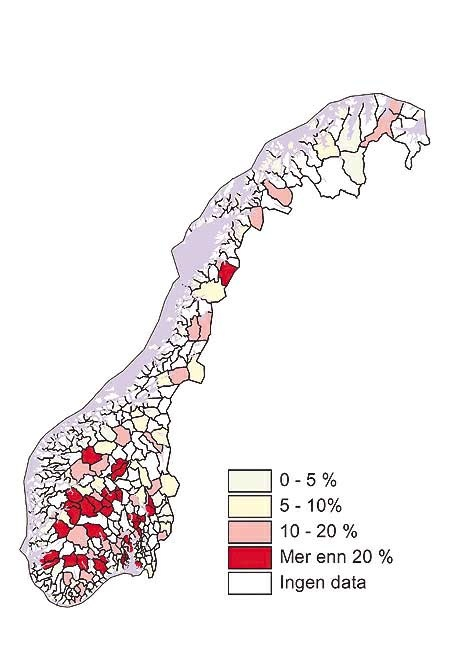
\includegraphics[width=90mm]{straleskart.jpg}
\caption{Oversiktskart. Prosenttallene angir hvor mange prosent over den anbefalte grensen på $200Bq/m^3$ det er funnet i boliger i disse områdene.
\textit{Kilde: Statens strålevern}
}
\label{fig:oversiktskart}
\end{figure}


\subsubsection{Produktkonsept}

Det nye produktet kommer av en ny teknologi fra CERN. Teknologien gjør at det er enklere og raskere å måle alfapartikler. Som sagt tidligere kunne en prøve ta opptil 10 minutter, men med den nye sensoren kan man få resultatene i sanntid. Dette fører til en mye mer effektiv måleprosess, hvor man vil bruke mindre av arbeidstiden til å utføre målingene. Med dagens radonsniffere vil man kunne bruke f.eks en time på en diagnosejobb, mens med dette nye produktet vil samme jobb kunne gjøres på 20 minutter. Samtidig skal denne måleren være mye mer pålitelig en de som nå er på markedet. Man skal ikke trenge å få problemer med apparatet, som at man må lufte det.	

Tanken med dette produktet er å ha en webapplikasjon til produktet. Når man utfører en måling skal det være mulig å legge inn måledataen trådløst inn på en datamaskin, som gjør at det blir enklere og aksessere og tolke informasjonen. Samtidig vil det gjøre at man lettere har informasjonen tilgjengelig til senere om det trengs, det vil være lettere å oppdatere hvordan konsentrasjonsnivået av radongass er og man vil ha mulighet til å utnytte måledataene på en helt annen måte. Det skal senere være mulig å vise informasjonen på et kart. Tanken er at når måledataene blir lagt inn på computeren, vil kartet bli oppdatert automatisk, med informasjon som gps-lokasjon, dato og strålemengden. En annen mulighet som også er mulig, er at selve måleren laster opp måledataen rett opp til nettapplikasjonen, som igjen bruker informasjonen til å direkte oppdatere og legge til den nye informasjonen.

\subsubsection{Utfordringer med produktet}

For å få produsert måleren, skal det kjøpes inn deler fra utlandet, de skal sendes til Norge og bli satt sammen her. Dette gjøres for å sikre at kvaliteten blir tilfredsstillende. En av utfordringene blir å designe elektronikken. Noe man må undersøke mer er hvor vanskelig det vil være å integrere mobilteknologi, som gjør det mulig å laste opp data direkte til skyen, uavhengig av en datamaskin med internettilgang. Systemet må bli programmert slik at det kan koble til internett og laste opp målingene. Teknologien, iallfall elektronikken, som produktet trenger finnes allerede. Jobben ligger i å designe de elektroniske kretsene, programmere mikroprosessoren og utforme selve produktet med et robust kabinett og det hele.

Det har tidligere vært noen få problemer med den nye sensorteknologien. Da de brukte den til forsøk i CERN, kunne det oppstå støy og feilaktige målinger (den detekterte alfapartikler når det egentlig ikke var noen der). Det har vært jobbet en del med å finne ut av hva grunnen til dette var. I etterkant viste det seg at grunnen til dette var støy på selve strømkilden, så dette har allerede blitt fikset og er ikke lenger noe problem.

Utfordringer kan også komme ved utvikling av webapplikasjonen som er tiltenkt dette produktet. Her er det mange spørsmål i forhold til om informasjonen skal lastet rett opp på skyen, om det skal legges lokalt først. Mye av utfordringen handler om hva som kan være best og enklest med tanke på at all informasjonen kanskje ikke skal bli offentlig for alle men for individuelle brukere. Om deler av dataene ikke skal bli offentlige for noen for eksempel. Det er mange vanskeligheter som må tas opp og se gjennom så det ikke brytes noen retningslinjer eller lover.
